%% template for IEICE Transactions
%% v1.7new [2010/02/03]
\documentclass[paper]{ieice}
%\documentclass[invited]{ieice}
%\documentclass[survey]{ieice}
%\documentclass[invitedsurvey]{ieice}
%\documentclass[review]{ieice}
%\documentclass[tutorial]{ieice}
%\documentclass[letter]{ieice}
%\documentclass[brief]{ieice}
\usepackage[dvips]{graphicx}
\usepackage[fleqn]{amsmath}
\usepackage[varg]{txfonts}
\usepackage{url}
\usepackage{cite}
\usepackage{epsfig}
\usepackage{float}
\usepackage{caption}
%\usepackage{subcaption}
\usepackage{graphicx}
%\usepackage[ngerman]{babel}
%\usepackage[T1]{fontenc}
%\captionsetup[subfigure]{labelformat=parens, format=hang, margin=0pt, parskip=0pt,
%		hangindent=0pt, indention=0pt, singlelinecheck=false, textfont=footnotesize}

\setcounter{page}{1}
%\breakauthorline{}% breaks lines after the n-th author

\field{B}
%\SpecialIssue{}
\SpecialSection{on XXXYYYZZZ}
%\theme{}
\title{P2PCDN}
%
%\title[title for header]{title}
\authorlist{% fill arguments of \authorentry, otherwise error will be caused. 
 \authorentry[dikshie@sfc.wide.ad.jp]{{Mohamad Dikshie} Fauzie}{n}{labelA}
 \authorentry{{Achmad Husni} Thamrin}{n}{labelA}
% \authorentry{Rodney Van Meter}{n}{labelB}
 \authorentry{Jun Murai}{m}{labelB}
}
\affiliate[labelA]{The author is with Graduate School of Media and Governance Keio University, Fujisawa-shi, 252-0882 Japan }
\affiliate[labelB]{The author is with Faculty of Environment and Information Studies Keio University, Fujisawa-shi, 252-0882 Japan }

%\paffiliate[present affiliate label]{Presently, the author is with the }
\received{2010}{1}{1}
\revised{2010}{1}{1}
%\finalreceived{2010}{1}{1}

%% <local definitions here>
%% </local definitions here>

\begin{document}
\maketitle

\begin{summary}
\end{summary}
\begin{keywords}
P2P, CDN, Internet Service Providers, Content Providers, Game Theory 
\end{keywords}  

%%%%%%%%%%%%%%%%%%%%%%%%%% INTRODUCTION %%%%%%%%%%%%%%%%%%%%%%%%%%%%%%%%%%%
\section{Introduction}\label{intro}
In recent years due to the widespread of broadband Internet connections, user achieved the possibility of downloading and sharing their multimedia contents.
Futhermore, more advanced hardware with a reduction of computer costs allowed users to own a high performance PC to perform complex task.
More people are watching video on their PC using specific applications or plugins that integrated into browsers.
Common technical solution just rely on a client-server architecture.
This solution is not viable since it can not scale if the content becomes popular.
Some content companies have agreement with CDN (content delivery network) providers such as Akamai, Limelight, or Level3 to distributed the contents better scale and better QoE (quality of experience) to end users.
For example, Youtube uses Google cache, MTV uses Akamai, etc. P2P (peer to peer) applications are also widely deployed and their success is quite important. 
In China, P2P is very popular. 
We see many P2P applications from China such as PPLive, PPStream, UUSe, Xunlei, etc.  
Some news broadcaster are also rely on P2P technology to deliver popular live events.
For example, CNN uses Octoshape solution that enable to scale and offer good video quality while the number of users increase.
From Internet provider point of view, the diffusion of powerful computers in users side suggested that it could be possible to delegate a portion of computing or storage tasks to the users thus creating P2P networks where users can share files and multimedia contents.
Starting from file sharing only protocol, P2P architecture evolved toward video on demand and live events support. 

A P2P based architecture usually requires a sufficient number of nodes supplying the data (termed as seeders) to start the distribution process among the joining peers.
A peer usually offers low outbound streaming rate due to traditional asymmectrical DSL home connections) and hence multiple peers must jointly stream a media data to a requesting peer. 
The decentralized, uncoordinated operation implies that scaling to high number of peers comes with side effects.
Typical problem of a P2P streaming architecture are the low stream quality with undesirable disruptions, resources unfairness due to heteregeneous peer resources and high startup delay.
Moreover, current P2P applications are not aware of the underlying network and may conflict with the ISP routing policies and business model.

Nowadays, a number of P2P streaming applications have been designed, analyzed and deployed attracting a significant amount of users.
Research studies and deployement experiences have both demostrated that P2P is a promising solution in terms of scalability and deployment costs.
On the other hand, the heteregeneous nature and unstable behavior of the peers contributing bandwidth and computational resources along with the networking issues are limit the commercial success of P2P video streaming applications.
Apart from P2P protocols, video contents can be efficiently distributed leveraging on services offered by managed networks architectures and CDN companies.
The major issue of CDN are high deployment cost and limited scalability in the long term.
Given the complementary features of P2P and CDN, in the last years some hybrid solutions have been proposed \cite{Huang:2008:UHC:1496046.1496064,4772628,Yin:2009:DDH:1631272.1631279} to take the best of both approaches.

Nowadays, xDSL networks are deployed worldwide and broadband acess network helps the P2P application to perform better.
In the coming years, FTTH will be massively deployed by network operators in order to offer to their customers and even larger acces bandwidth.
As bandwidth increase, more the P2P systems is efficient since a peer can contribute much more. 

P2P architecture offers great potential for content providers to cost effectively distribute content by capitalizing network resources of end users.
It is economical superiority to the traditional client-server architecture and it has been demonstrated by lots of academic work and successful commercial systems \cite{Yin:2009:DDH:1631272.1631279}.
We believe more content providers will adopt P2P technology in the future. 

In the mentioned work, each end user device is involved directly in the P2P swarm.
In such cases, the installation of a software for the P2P engine in every end device is necessary and the user itself is directly involved in the content's swarm.
In such condition peers may result unstable and the swarm can be affected by rapid and frequent disconnections.
Furthermore, user's devices usually can contribute to the swarm with limited upload bandwidth and techniques developed in P2P to select neighboring peers are often unfriendly with ISP's routing policies.
Different topologies have been proposed in literature, where the collaborative mechanism for content distribution is created among more stable devices such as residential gateways which are still geographically close to the end users but directly owned and managed by ISPs. 
In such conditions, running on more stable and powerful device, each peer can contribute with more bandwidth to the content swarm with respect to traditional end-user P2P. 
Peer selection procedures can also managed directly by ISP, avoiding the traversal of multiple nodes across ISP boundaries.

In some recent works, the residential gateway (i.e a home gateway placed in home premise, serving several terminals within the home network but directly managed by ISP) is considered the central entity of such managed P2P infrastructure as describe in \cite{Misra:2010:IPS:1811099.1811064,Cha:2008:NTP:1855641.1855646}.
Since P2P traffic now decreasing and moving to cloud \cite{Labovitz:2010:IIT:2043164.1851194}, there is room from ISP to use user's home gateway as peer assisted CDN since users usually do more download rather than upload.
The user home gateway is always on 24 hours therefore this is perfect device to run peer assisted application.
ISP can give discount price to user's who wants their home gateway to be used as peer assisted by ISP and ISP can get benefit from peer assisted running in their customer home gateway to help their CDN.
With the growing interest to do inter-connect of CDN \cite{cdni,oceanproject} this architecture can give good benefit for ISP.    

In this paper we study, the economic incentive for ISP who adopt peer assisted CDN and shows that the advantages to adopt peer assisted CDN. 
%We use single shot game theory to model of the balance between ISP profit that get from employed peer assisted CDN and traffic saving. 

%\begin{figure}[tb]
%\begin{center}
%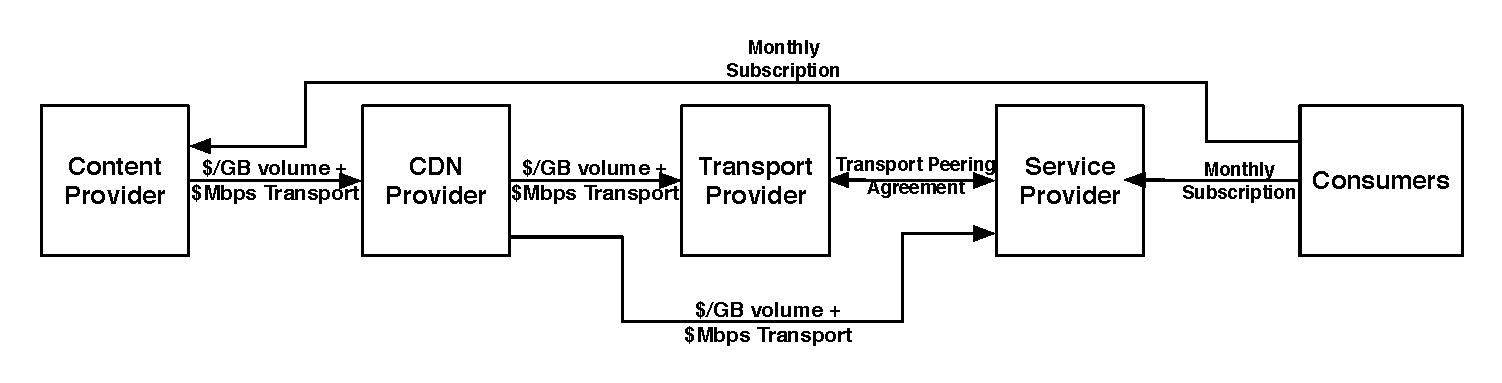
\includegraphics[scale=0.35]{graphs/today-ecosystems.eps}
%\end{center}
%\caption{Today Ecosystems.}
%\label{fig:todayeco}
%\vspace{-2mm}
%\end{figure}


%\begin{figure}[tb]
%\begin{center}
%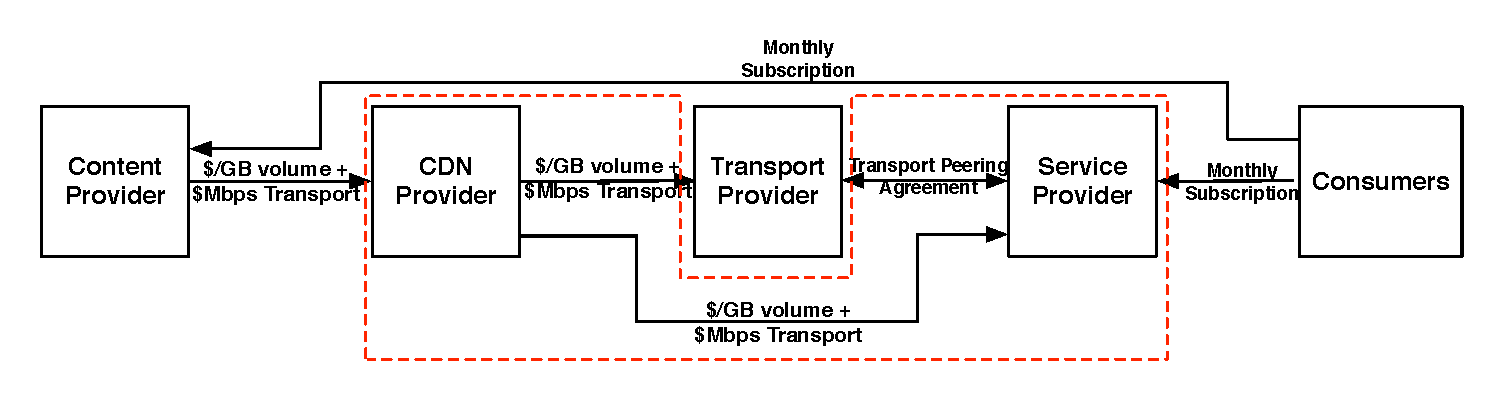
\includegraphics[scale=0.35]{graphs/today-ecosystems-sp.eps}
%\end{center}
%\caption{Today Ecosystems SP.}
%\label{fig:todayecosp}
%\vspace{-2mm}
%\end{figure}


\begin{figure}[tb]
\begin{center}
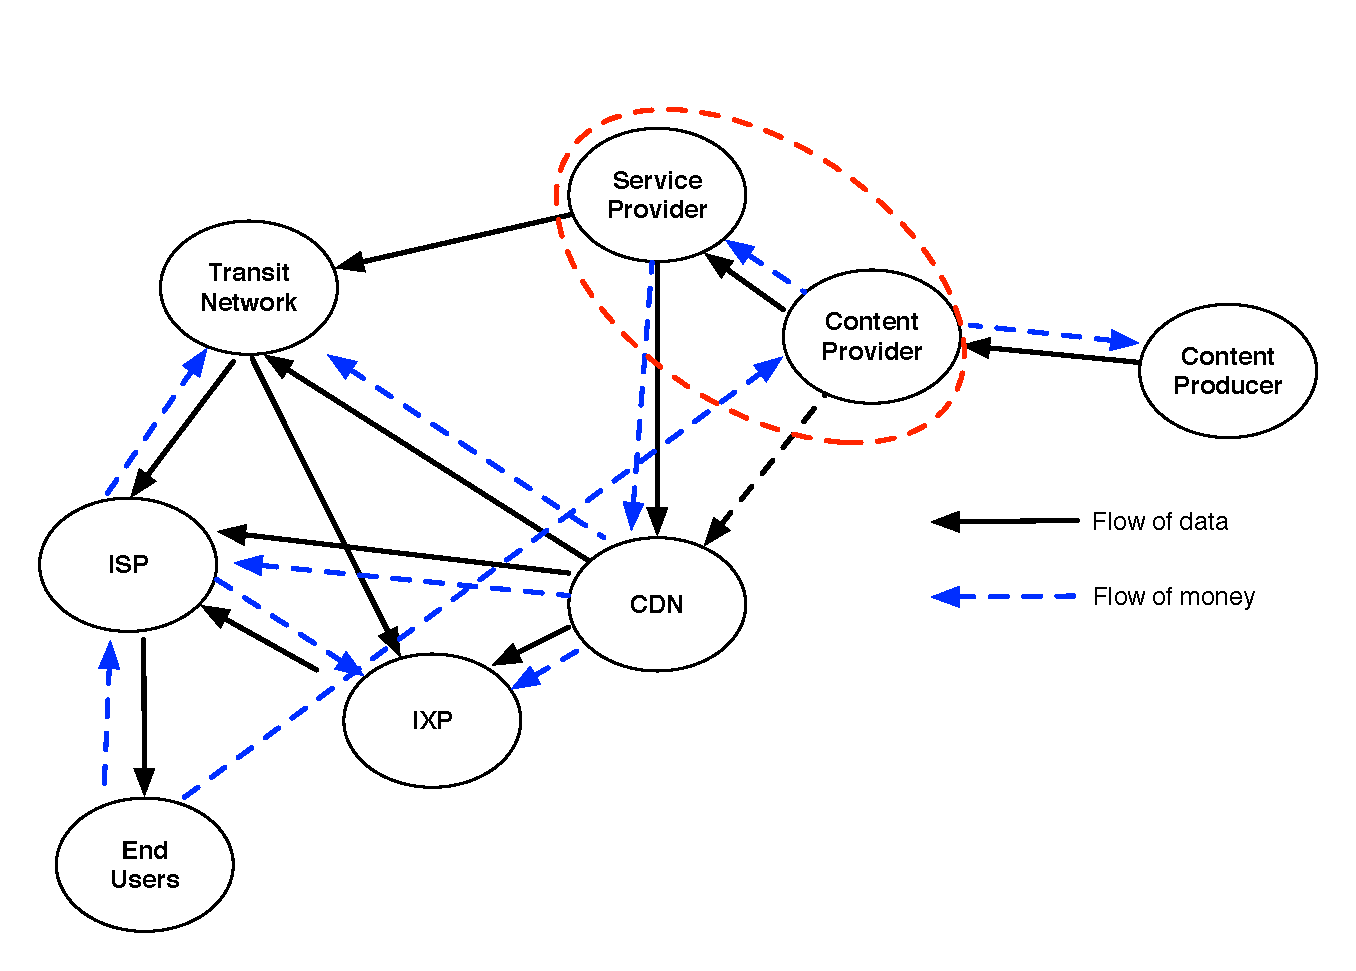
\includegraphics[scale=0.35]{graphs/business-relationship.eps}
\end{center}
\caption{Complex relationship of entities in Internet.The data flow from content producer to content provider. From content provider data can flow to service provider then goes to CDN. Depends on routing and peering policy, data from CDN can flow directly to ISP or flow to ISP via IXP (Internet Exchange) or via transit network. Flow of data noted by straight arrow and flow of money noted by dash arrow line.}
\label{fig:businessrelationship}
\vspace{-2mm}
\end{figure} 


%\begin{figure}[tb]
%\begin{center}
%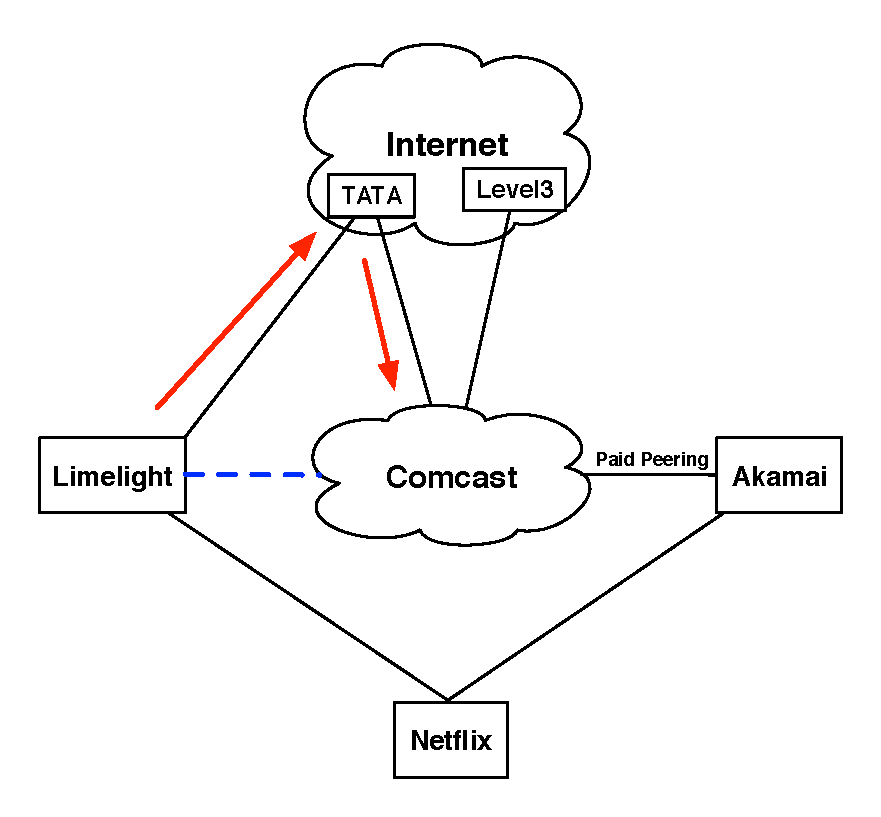
\includegraphics[scale=0.35]{graphs/llnw-tata-comcast.eps}
%\end{center}
%\caption{Akamai purchased paid peering from Comcast and enjoy low latency and high capacity access to Comcast's customers.
%Limelight use Tata to deliver contents to Comcast's customers (arrow line). 
%Due to high congestion on the link between Comcast and Tata, Netflix began to complain to Limelight because Netflix paid Limelight to deliver contents. 
%Finally Limelight purchased paid peering from Comcast (dash line).}
%\label{fig:llnw}
%\vspace{-2mm}
%\end{figure}

%\begin{figure}[tb]
%\begin{center}
%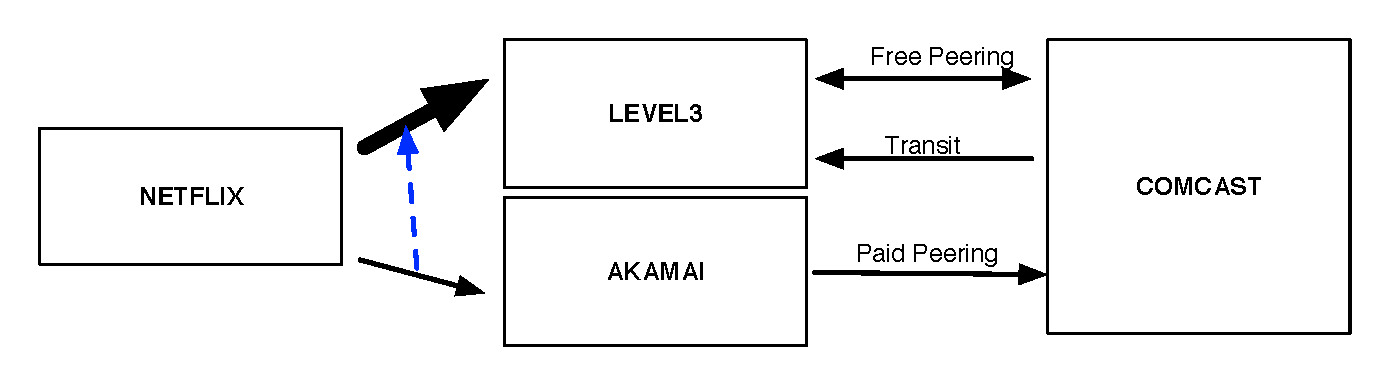
\includegraphics[scale=0.35]{graphs/comcast-level3.eps}
%\end{center}
%\caption{Level3 and Comcast has settlement free peering. Comcast is also use Level3 as transit network. 
%Netflix change its contents delivery network from Akamai to Level3 (arrow dash line).
%Level3 traffic to Comcast became out of ratio therefore Comcast asked Level3 to buy paid peering.}
%\label{fig:comcast}
%\vspace{-2mm}
%\end{figure}



%%%%%%%%%%%%%%%%%%%%%% CDN COMPLEXITY %%%%%%%%%%%%%%%%%%%%%%%%%%
\section{CDN Complexity}
As shown in Fig.\ref{fig:businessrelationship}, how content in Internet delivered to end-users.  
Content producer such as movies companies send their movies to content provider for example: Netflix and Hulu.
Content providers then deliver the movies using CDN or they also can use their upstream provider.
Depends on peering policies, CDN can reach to customer directly via ISP or via IXP then reach ISP or goes to transit networks then reach ISP.   
In current modern Internet topology, content provider and service provider can be merged in on entity, for example: Google.
Labovitz et al.,\cite{Labovitz:2010:IIT:2043164.1851194} mentioned that the hypergiant entities such as Google doing massive peering to IXP in order to be closed to ISP. 
Although CDN is placed close to ISP network, it does not guarantee end-users can get good quality video stream \cite{Krishnan:2009:MBE:1644893.1644917}.
Other than technical complexity as mentioned before, CDN also faces economic complexity.
Therefore, the future of CDN business is likely to live deeper into ISP networks, more integrated into and interleaved with ISP infrastructures.




%%%%%%%%%%%%%%%%%%%%%% SYSTEM DESCRIPTION %%%%%%%%%%%%%%%%%%%%%%%
\section{System Description}\label{description}

Fig.\ref{fig:twotier} shows the model of system archictecture.
That's model offers the opportunity to connect the P2P swarm not directly but through an intermediate later of proxies.
This function has potential benefit: boosting download performances (by exposing through proxy devices higher upload bandwidth than end users) and increasing privacy (by reducing swarm exposure for end users).
In Fig.\ref{fig:twotier} two level CDN is defined.
The first level L1 consists high capacity servers strategically placed to increase network backbone capacity.
L1 is more like current CDN network.
In L1 level, CDN node can communicate each other by using common interconnect interface eventhough the CDN node are owned by different companies or different ISPs \cite{cdni}.
L0 consists CDN proxies are owned or to be managed by ISP.
These nodes are placed closer to end users. 
CDN proxies can communicate each other to react to the content requests from users.
L0 are the natural service points for the users and they can offer the best quality of service if the are able to efficiently cache the requested content.
The state of the L0 and L1 caches is stored in DHT. 
The DHT is used to keep an updated record for each content in scalable manner. 
This different caching levels are used to offer an adaptive, flexible, and scalable service to the users.

Other architecture, CDN federation proposed by Cisco and some ISPs to interconnect the ISP's CDN \cite{federation}.
The goal this architecture is to interconnect ISPs owned CDN thus reduce Capex and Opex for content delivery. 
This architecture does not involved P2P. 
Some peering or transit might be needed by ISP to join this architecture. 
 
\begin{figure}[tb]
\begin{center}
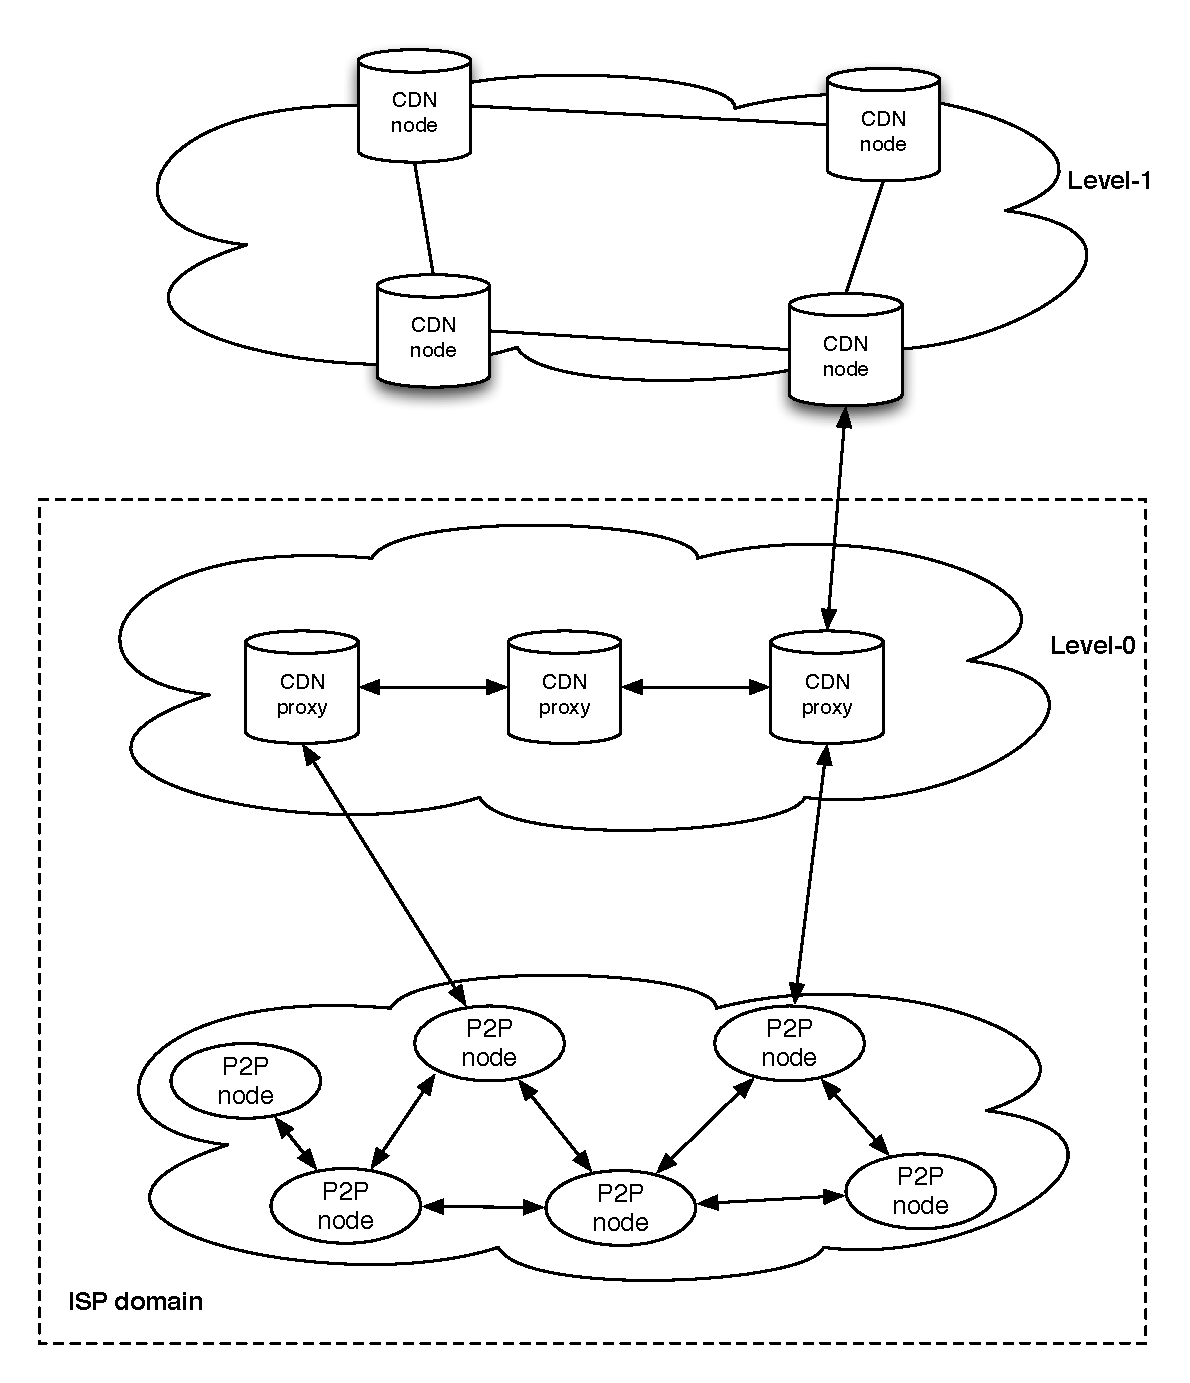
\includegraphics[scale=0.35]{graphs/two-tier-cdn-topology.eps}
\end{center}
\caption{Two tier CDN-P2P topology.
The CDN proxy maintained by ISP. ISP also has CDN node. CDN node can exchange contents with other CDN node owned by other CDN companies.P2P nodes are ISP's customers that run P2P software.}
\label{fig:twotier}
\vspace{-2mm}
\end{figure}
  
\section{System Model}\label{systemmodel}
We present a model between P2P and CDN using simple a single bitrate for video streaming as shown in Fig.\ref{fig:twotier2}. 
The model is a stochastic fluid model similar to \cite{4215694}.
While the authors in \cite{4215694} focus on probabiity of degraded service on small and large systems, our work focus on lower bound of peers that can support intended bit rate.
The knowledge of lower bound is very import for ISP to estimate number of customers that can join to P2P.
We aim to find out how many peers will be sufficient to provide a stream to a certain number of leechers.
Throughout the rest of this section we assume that CDN proxy has bit rate $r$  and the upload capacity of the CDN proxy is $C_{proxy}$.
On next subsection we also present a model of simple game theory between ISP who operate P2P-CDN and users.
We aim to find out the indifferent utility function between ISP and users.

\begin{figure}[tb] 
\begin{center}
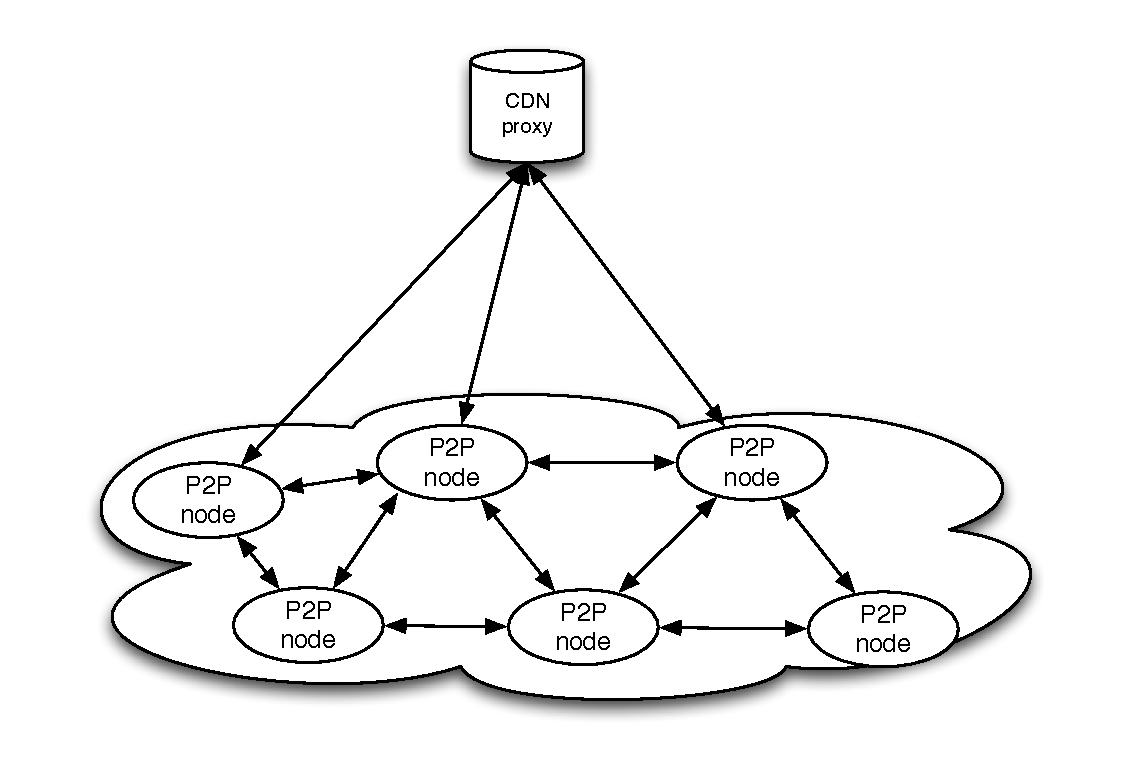
\includegraphics[scale=0.35]{graphs/two-tier-cdn-topology-2.eps}
\end{center}
\caption{System architecture on L0. P2P nodes that run on user homegateway communicates to CDN proxy.}
\label{fig:twotier2}
\vspace{-2mm}
 \end{figure}


We analyze the system for the theoretical unconstrained case when peers can have unlimited number of connections with other peers.
We also present the analysis more realistic case for constrained case when peers can only have a limited number of incoming and outgoing connections.
Moreover, for both case above we also present the analysis for churnless and churn systems.

For churn case, we assume peers join and leave at random times, stay in for a random period, then leave the system.
Assuming poisson process with rate $\lambda$.
Peers stay in the system for a period of time that follows a general probability distribution with mean $\frac{1}{\gamma}$.
Define $N(t)$ as the number of peers in the system at time $t$, $N(t)$ can be represented as the number of peers in a $M/G/\infty$ queue.

\subsection{Unconstrained System}
In unconstrained churnless system, denote $n_l$ is the number of leechers and $n_s$ is the number of seeders in the system.
Also denote $u_{i}^{l}$ , $u_{j}^{s}$ as upload rate of leecher $i$ and seeder $j$.
Following two condition must be holded: $C_{proxy}\ge n_s r$ and $\sum_{j=1}^{n_s} u_{j}^{s} \ge r$.
First inequality express server capacity constraint and second inequality express the set of seeders have minimum upload capacity.
The maximum achievable streaming rate $r_{max}$is given by
\begin{equation}
	r_{max} = min \{ {{U_s},\frac{U_s + \sum_{i=1}^{n_l} u_{i}^{l}}{n_l}} \}
\end{equation}
$U_s$ is total update rate of all seeders and $U_s=\sum_{j=1}^{n_s}u_{j}^{s}$
for simplicity we assume all leechers have the same upload rate of $u_l$ and all seeders have the same upload rate of $u_s$ thus $u_l$ and $u_s$ can be considered as the average upload rates over all leechers and seeders.  
we assume $r \ge u_l$. it means that the average upload rate of single leecher is not enough to support sharing the whole stream with other peers.
in that case $r_{max}$ can be reduced to $r_{max}=min\{n_s u_s,\frac{n_s u_s + n_l u_l}{n_l}\}$. 
when the system in the steady state condition we can assume that $n_s u_s \ge \frac{n_s u_s + u_l u_l }{n_l}$ then we can get that a churnless system can support 
a streaming rate of:
\begin{equation}
	r \le \frac{n_s u_s + n_l u_l}{n_l}
\end{equation}
we can derive for theoretical lower bound $n_s \ge \frac{n_l(r-u_l)}{u_s}$ on the number of seeders to support bitrate $r$.

In unconstrained with churn system, denote $N(t)$ is the total number of peers in the system at time $t$ (including seeders and leechers) and $N$ follows a Poisson distribution with rate $\rho = \frac{\lambda}{\gamma}$.
for computing the probability that the system will be able to support a streaming rate $r$ in case of node churn, we assume that node churn only happens in leecher nodes. This means number of seeders in the system are assumed to be constant. Only leechers arrive and leave the system.
The probability that we can support a bitrate $r$ as following:
\begin{align*}
  P(r) &= P(r \le \frac{n_s u_s + N u_l}{N}) \\
  &=P(N \le \frac{n_s u_s}{r - u_l}) \\
  &=F(\frac{n_s u_s}{r - u_l})
\end{align*}

$F(w) = \sum_{x=0}^{w}\frac{e^{\rho}\rho^{x}}{x!}$ for large system we can assume $\rho \rightarrow \infty$ thus we can approximate the Poisson distribution with a Gaussian distribution with mean $\mu = \rho$ and standard deviation $\sigma = \sqrt{\rho}$ as $\frac{1}{\sigma}\phi(\frac{x-\mu}{\sigma})$.
Hence, we can get:
\begin{align*}
	P(r) &= P(\frac{N-\rho}{\sqrt{\rho}} \le \frac{\frac{n_s u_s}{r - u_l}- \rho}{\sqrt{\rho}}) \\
	&= \Phi(\frac{ \frac{n_s u_s}{r - u_l} - \rho}{\rho})
\end{align*}
$\Phi(z)$ is the cumulative distribution function of the standard normal random variable.
Let $\phi_{1-\alpha}=1 - \alpha$ where $\phi_{1-\alpha}$ is a positive real number.
The confidence $(1-\alpha) x 100 \%$ that peers can support bitrate $r$ is $(\frac{n_s u_s}{r - u_l} - \rho)/ \sqrt{\rho} \ge \phi_{1-\alpha}$.
Finally we can derive lower bound on the number of peers:
\begin{equation}
	n_s \ge \frac{(\phi_{1-\alpha} \sqrt{\rho} + \rho)(r - u_l)}{u_s}
\end{equation}

\subsection{Constrained System}
In constrained system, each peer as a limited number of inbound and outbound connections. 
We defined the limit as following:
\begin{itemize}
	\item $S_{in}$ is the maximum number of incoming connections a seeder can accept.
	\item $Y_{in}$ is the maximum number of incoming connections a leecher can accept.
	\item $Y_{out}$ is the number connections a leecher can initiate. We assume that there is no limit on the number of connections a leecher can initiate.
	It means the bottleneck is in the number of connections that actually established. 
	This number is mainly controlled by parameter $S_{in}$ and $Y_{in}$
\end{itemize}

We define $\eta$ as the efficiency of the P2P protocol which can be computed as the probability of any leecher finding new content at other leechers when they establish a connection \cite{Qiu:2004:MPA:1030194.1015508}.
It is shown that Bittorrent efficiency can exceed $0.9$ if the file has more than ten pieces \cite{4199285}.
P2P protocol efficiency means that a leecher has an effective upload rate of $\eta u_l$.
Denote $d$ as the average download rate for any leecher in the swarm, then $d$ can be computed as:
\begin{align*}
	d &= \sum_{x} E[d] | \text{leecheer connected to x seeders}] \times P_r\{x\} \\
	&= \sum_{x} (\frac{xu_s}{S_{in}} + \frac{(Y_{out}-x) \eta u_l}{Y_{in}}) P_r\{x\} \\
	&= \frac{Y_{out} \eta u_l}{Y_{in}} + ( \frac{u_s}{S_{in}} - \frac{\eta u_l}{Y_{in}} ) \sum_x x Pr\{x\}
\end{align*}

Note that $\sum_x s Pr{x}$ is the average number of seeders connected to each leecher which can be approximated by the value $n_s S_{in}/n_l$.
Note also that when $n_l \ge n_s$, we can calculate an approximate value for the number of connections each leecher can establis by $Y_{out} = (n_s S_{in} + n_l Y_{in})/n_l$. 
Subtituting these two equations in equation above , then $d$ can be reduced to:
\begin{equation}
	d = \frac{n_s u_s + \eta n_l u_l}{n_s}
\end{equation}
Since $d$ can be considered the average bitrate that can be supported by the system, then the number of seeders sufficient to support the bitrate is $n_s = n_l (r -\eta u_l) / u_s$. 

In constrained system with churn, we can compute the probability of supporting a range of bitrates $r$ in a system as follows:
\begin{align*}
	P(r) &= P(\frac{n_s u_s + \eta N _ul}{N} - \delta \le r \le \frac{n_s u_s + \eta N u_l}{N}+\delta) \\
	P(r) &= P(\frac{n_s u_s}{r - \eta u_l + \delta} \le N \le \frac{n_s u_s}{r - \eta u_l - \delta})
\end{align*}
As we did earlier, $N$ can be approximate by a Gaussian random variable. 
With $(1-\alpha) 100\%$ confidence interval for $N$ we can set:
\begin{equation*}
	\frac{ \frac{n_s u_s}{r - \eta u_l + \delta} - \rho }{\sqrt{\rho} } \le - \phi_{1-\alpha/2} , \frac{ \frac{n_s u_s}{r - \eta u_l - \delta} - \rho }{\sqrt{\rho} } \ge \phi_{1-\alpha/2}
\end{equation*}
We define $\hat{\phi}=\phi_{1-\alpha/2}$ then we can get following confidence interval for $N$
\begin{equation*}
	\frac{ (\rho + \hat{\phi} \sqrt{\rho} )(r - \eta u_l - \delta)}{u_s} \le n_s \le \frac{ (\rho - \hat{\phi} \sqrt{\rho} )(r - \eta u_l + \delta)}{u_s}
\end{equation*}
This inequality provides valid intervals only for $\delta$ values that satisfy the condition $\delta \ge \frac{\phi_{1-\alpha/2} (r - \eta u_l)}{\sqrt{\rho}}$.
We can see that $\delta$ is inversely  proportional to $\rho$. 
It means that the higher peer arrival rates and the longer peers stay in the system, the lower $\delta$ becomes.
Lower $\delta$ mean a smaller interval in inequality which yiedls a higher guarantee that the number of peers given by above interval will be sufficient for supporting the bitrate $r$. 


\subsection{ISP Strategies: Game Theory Approach}
In this section, we present simple game theory approach for analysis of ISP strategies.
Game theory as described in \cite{gametheory} is a mathematical framework to study and analysis of situation where decisions made by a set of two or more rational players.
Basic element of game are: rational players, strategies, and payoff or utility.  
Rational players choose a strategy for maximizing its payoff or utility. 
Extensive-form game is representation of corresponding decision nodes in a directed tree.
Later, we will use extensive-form game to represent our game.
In our model, ISP has already attempted to implement solution for peer-assisted CDN.
Moreover, it is reasonable to assume that ISP is naturally initiators.  
Stackelberg game also known as a leader-follower game is a class of game that concerns with situation where one player, the leader, initiates the decision making and where the second player, the follower, responds to the actions by the leader.  
Moreover in our model, ISP can be modeled as leader who decided to implement peer-assisted or not according to their expected payoff, while users can be modeled as followers that evaluate the decision of the ISP and responds according to their available actions and payoffs.

\newtheorem{theorem}{Definition}
\begin{theorem}[ISP Strategies]
We define the pure strategy space $S_{isp}$ to include two strategies combination choice $s \in \{No, P2P\}$ and corresponding subscription free $P^{s}$.
Futhermore, we denote the strategies as:
\begin{itemize}
	\item $s_1 = (No, P^{s_1})$ : the ISP decides to do nothing (use CDN only) and thus keeps charging the initial subscription free $P^{s_1}$.
	\item $s_2 = (P2P, P^{s_2})$ : the ISP decides recommends P2P and offers a subscription fee $P^{s_2} \le P^{s_1}$.
\end{itemize}
Where the ISP strategy space $S_{isp} = \{s_1,s_2\}$.
\end{theorem}

After defined the strategy space of ISP, now we will describe user reaction.
One obvious user action is to accept ISP strategy.
When user receives offer from ISP whether user want to join peer-assisted strategy or not to join peer-assisted strategy, user can only accept one of that strategy.  
If user decides to join P2P strategy from ISP then it means user accept $s_2$ of ISP.
If user decides not to join P2P strategy from ISP then it means user accept $s_1$ of ISP.
Therefore whatever strategy offered by ISP, the user can only accept one of the ISP strategy.

\newtheorem{theorem2}{Definition}
\begin{theorem}[User Strategies]
Given a ISP strategy decision $s$, we define the user action as $s_a$ where user accepts ISP strategy $s \in S_{isp}$.
\end{theorem}
We describe that situation as extensive form in Fig.\ref{fig:gametree}.



\begin{figure}[tb] 
\begin{center}
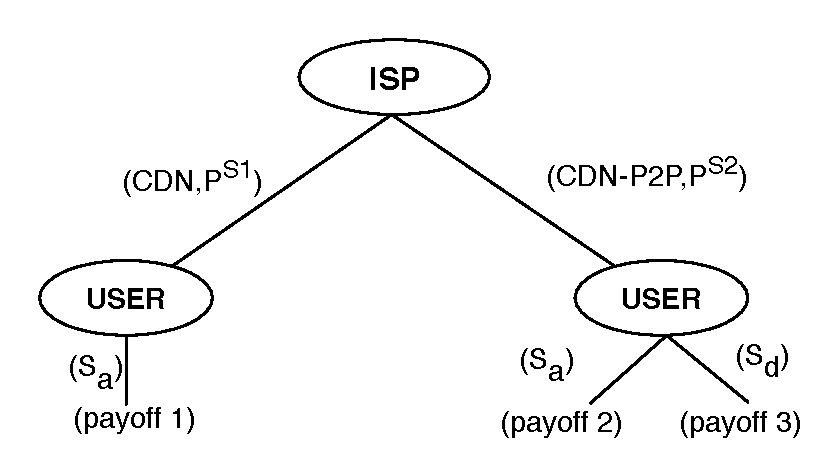
\includegraphics[scale=0.35]{graphs/game-tree.eps}
\end{center}
\caption{Extensive form of game between ISP and users}
\label{fig:gametree}
\vspace{-2mm}
\end{figure}

\subsubsection{ISP Payoff}
Next, we describe payoff function for ISP in our model.  
We assume a profit maximaxing ISP that gains higher utility proportionally with increasing profits. 
A simplified business model that determining ISP payoff are mainly: user generated revenue and traffic cost from inter ISP traffic (transit and peering).

For revenue model, we assume that the ISP collects revenue solely by charging an initial flat rate subscription fee $P^{(s_1)}$ to its $N$ homogeneous users who are purchasing internet access with equal and fixed quality of service.
ISPs are often price discriminatory towards its customers and thus operates with different price levels for different speed or QoS.
ISPs are also get revenue from other business area such as email hosting, web hosting, etc. 
In our model, we do not include such that revenue. 
In order to keep simple, we found it reasonable only to focus on users that buy the same internet access product. 
Given above simplifications, the ISP collects a total revenue (when deciding on a strategy $s$) of $R = N P^{(s)}$.

For cost model, we identified that traffic costs including (transit traffic and paid peering) are the most relevant aspect. 
\newtheorem{theorem3}{Definition}
\begin{theorem}[Transit cost]
we define the transit cost $\tau^{(s)}$ for a given ISP strategy $s$ to be denoted as 
\begin{equation}\label{eq:transitcost}
	\tau^{(s)}_t = \alpha^{(s)} \beta T^{(s_1)} p_t
\end{equation}
where:
\begin{itemize}
	\item $T^{(s_1)}$ represent the average inter-ISP traffic volume in Mbps.
	\item $\alpha^{(s)}$ represent the expected reduction factor of inter-ISP traffic for strategy $s$ such that: $\alpha^{(s)} \in [0,1]$ for $s \in \{s2\}$;  $\alpha^{(s_1)} = 1$.
	\item $\beta$ represent the ratio of inter-ISP traffic volume $T^{(s)}$ that traverse transit links such that: $\beta \in [0,1]$.
	\item $p_t$ represent the price of transit traffic.
\end{itemize}
\end{theorem}

\newtheorem{theorem4}{Definition}
\begin{theorem}
We define the paid peering traffic cost $\tau^{(s)}$. 
Paid peering costs are subject to a peering traffic price $p_p$.
Futhermore, as $\beta$ is the ratio of the inter-ISP traffic $T^{(s)}$ that traverses transit links, $(1-\beta)$ express the ratio that traverses paid peering links.
We can denote the paid peering traffic cost as:
\begin{equation}\label{eq:paidpeeringcost}
	\tau^{(s)}_p = \alpha^{(s)} (1-\beta) T^{(s_1)} p_p
\end{equation}
\end{theorem}

newtheorem{theorem5}{Definition}
\begin{theorem}
Given transit cost and paid peering cost in Eq.\ref{eq:transitcost} and Eq.\ref{eq:paidpeeringcost}, we can define total inter-ISP traffic cost $\tau^{(s)}$ as:
\begin{align}
	\tau^{(s)} &= \tau^{(s)}_t + \tau^{(s)}_p \\
	\tau^{(s)} &= \alpha^{(s)} \beta T^{(s_1)} p_t + \alpha^{(s)} (1-\beta) T^{(s_1)} p_p
\end{align}
\end{theorem}

In addition to the traffic costs, we also assume that ISP needs investment cost for peer-assisted CDN.
More specifically refer to Fig.\ref{fig:twotier2} ISP required to setup their L0 or CDN proxy.

\newtheorem{theorem6}{Definition}
\begin{theorem}
We define the investment cost $C^{(s)}_i$ to be a monthly amortization of a larger implementation related cost for the case when the ISP decides to implement P2P. 
We denote:
\begin{align}
	C^{(s)}_i &\ge 0; \text{ for } s = s_2 \\
	          &= 0; \text{ for } s \in \{s_1\}
\end{align}
\end{theorem}

Finally after we defined all ISP cost, we can define ISP payoff funtion that will be used to model ISP utility.  

\newtheorem{theorem7}{Definition}
\begin{theorem}
We define the ISP payoff function $\pi_{isp}$ as:
\begin{align}\label{eq:isppayoff}
	\pi_{isp}^{(s)} &= N P^{(s)} - \tau^{(s)} - C_i^{(s)} \\
	 &= N P^{(s)} - \alpha^{(s)} \beta T^{(s_1)} p_t + \alpha^{(s)} (1-\beta) T^{(s_1)} p_p - C_i^{(s)} 
\end{align}
\end{theorem}

\begin{figure*}[tb]
\begin{minipage}[b]{0.4\linewidth}
\centering
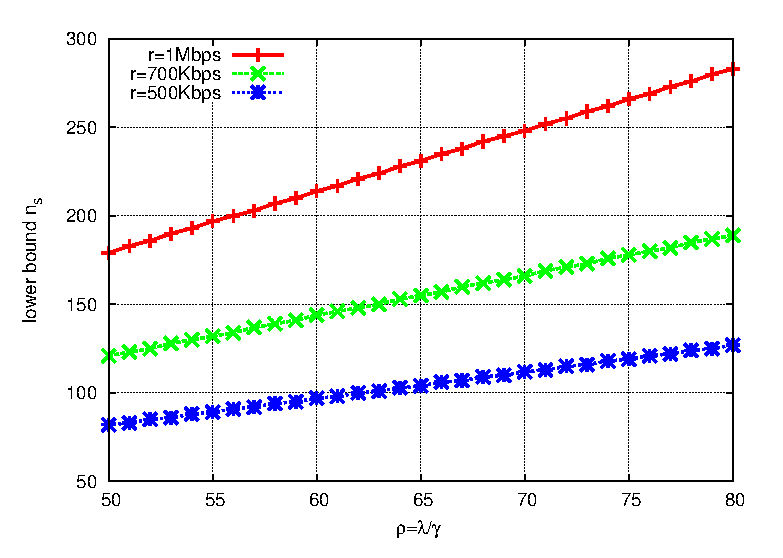
\includegraphics[width=2.7in]{graphs/constrained.eps}
\caption{Constrained system with churn, 95\% confidence}
\label{fig:cons}
\end{minipage}
\hspace{0.5cm}
\begin{minipage}[b]{0.5\linewidth}
\centering
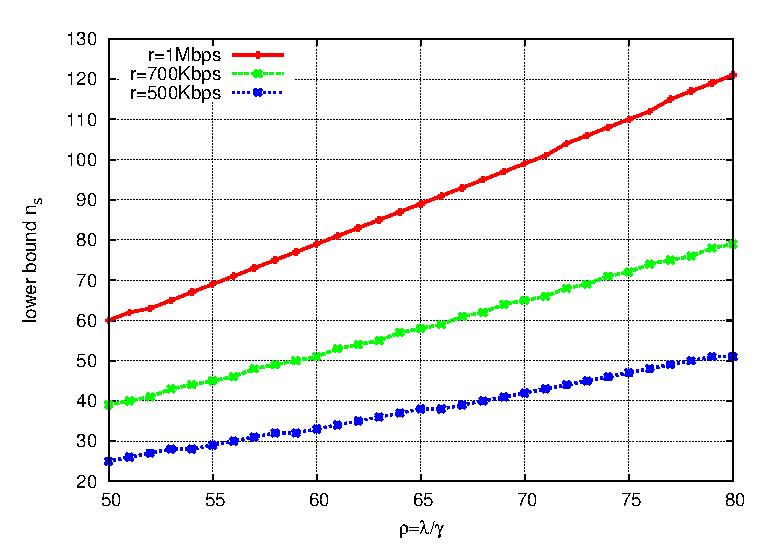
\includegraphics[width=2.7in]{graphs/unconstrained.eps}
\caption{Unconstrained system with churn, 95\% confidence}
\label{fig:uncons}
\end{minipage}
\end{figure*}
 
\subsubsection{User Payoff}
In this subsection, we  analyzed how the utility of user that purchases internet access at a fixed subscription fee $P^{(s)}$ can be described and derived. 
We assume that all users pay a fixed flat rate subscription fee $P$ for internet access with equal speed or QoS parameters.
Since users are rational player and subject to budget constraint, there must be a set of feature of internet access that valuable to users.
We assume one important parameter that describes the quality of an internet access product as perceived by customer is the perceived performance of internet applications.  
Moreover, the implementation of peer assisted mainly to reveal improvements of download speed as the performance metric that can be observed by customers.
Consequently, we make assumption that the user perceived quality of internet access increases proportionally with increases in peer assisted implementation. 

\newtheorem{theorem8}{Definition}
\begin{theorem}
we define the user perceived quality $Q^{(s)}$ of the internet access given an ISP strategy $s$ to be a function of the experimental derived peer assisted performance improvement $d^{(s)}$ that corresponds to $s$. 
Moreover it is assume that the user initially perceived quality $Q^{(s_1)}$ is known. 
We formally denote $Q^{(s)}$ as:
\begin{equation}\label{eq:basicuserutility}
	Q^{(s)} = Q^{(s_1)} (1 + d^{(s)})
\end{equation}
\end{theorem}

Therefore, given the assumption of proportional utility contribution from quality and price, we can define basic utility $U^{(s)}$. 

\newtheorem{theorem9}{Definition}
\begin{theorem}
We define basic utility $U^{(s)}$ a customer receives from buying internet access, given asn ISP strategy decision $s$ as:
\begin{equation}
	U^{(s)} = Q^{(s)} - P^{(s)}
\end{equation}
Where $Q^{(s)} > P^{(s)}$.
\end{theorem}

Finally, General form user payoff function (user accepts ISP strategy $s$):
\begin{equation}
	\pi^{(s_a | s)}_u = U^{(s)}
\end{equation}
by subtitution basic user utility in Eq.\ref{eq:basicuserutility}, we can get general user payoff function:
\begin{equation}
	\pi^{(s_a | s)}_u  = Q^{(s_1)} ( 1 + d^{(s)}) - P^{(s)}	
\end{equation}


%%%%%%%%%%%%%%%%% SECTION ANALYSIS & DISCUSSION %%%%%%%%%%%%%%%%%
\section{Analysis and Discussion}

\subsection{Constrained and Unconstrained System}

Figure \ref{fig:cons} shows numerical results of lower bound for seeders againts $\rho$ for constrained system with churn and Fig.\ref{fig:uncons} shows numerical results of lower bound for seeders againts $\rho$ for unconstrained system with churn.  
Both numerical results have 95\% confidence interval on the number of seeders sufficient to support bitrate $r$.  
We use $1/\gamma = 0.5$ hour thus we suppose that peers sojourn in the system on average for 30 minutes and we fix the arrival rate of the peers to $\lambda=100$ per hour.
We increase arrival rate $\lambda$ until $160$ per hour. 
We can see that the difference in the number of seeder sufficient to support different bitrates is not large.  
We also see that that lower bound number for seeders is very easy to fullfil by ISP to employ system because ISP's customer number much higher that that lower bound.

\subsection{Analytical Equilibrium Analysis}
As defined in previous section, both users and ISP are modeled as selfish players that maximize their utility (payoff) defined in the payoff functions.
As a consequence, an incentivizing strategy for both users and ISPs is a strategy that yields higher payoff then the other available strategies.
The ISP cacting as a leader and initiator of the decision making, decides, on strategy $s$ that includes both a choice of technology as well as price offer $P^{(s)}$ which affect both ISP and user payoff.

From the user payoff function, we observe that a user receives higher payoff as price decreases and will prefer lower prices.
The ISP on the other hand will naturally have a minimum limit for the subscription price as it, in our model, represents the only source of revenue.
Moreover we say that the minimum price $P^{(s)}_{min}$ that makes an ISP indifferrent between strategy $s \in \{s2\}$ and strategy $s_1$ can be found by identifying where the payoff of strategy $s$ equal the payoff of strategy $s_1$. 
That is expressed formally as:
\begin{equation}\label{ispminprice}
	\pi^{(s)}_{isp} = \pi^{(s_1)}_{isp}
\end{equation}
Where $s \in \{s2\}$. 
Later Eq.\ref{ispminprice} can be written as: 

\begin{equation}\label{eq:ispminprice2}
	N P^{(s)}_{min} - \tau^{(s)} - C^{(s)}_i = N P^{(s_1)} - \tau^{(s1)}  
\end{equation}
When subtituting payoffs with Eq.\ref{eq:isppayoff}, by furthermore solving Eq.\ref{eq:ispminprice2} for $P^{(s)}_{min}$ we can get:
\begin{equation}\label{eq:ispminprice3}
	P^{(s)}_{min} = P^{(s_1)} - \frac{1}{N} ( \tau^{(s1)} - \tau^{(s)} -  C^{(s)}_i  )
\end{equation}
Given the above equations, we have found an expression for $P^{(s)}$ that express the point at which the ISP is indifferent to strategy $s$ over $s_1$ and thus represent the lower boundary for where both the users that ISP might have incentives for strategy $s$. 
Above equation also express that ISP at maximum are willing to reduce its initial price $P^{(s_1)}$ by the expression $\frac{1}{N} ( \tau^{(s1)} - \tau^{(s)} -  C^{(s)}_i  )$.
Moreover it can be interpreted as a combination of the reduction in ISP total costs and investment.
Naturally, the implementation of peer assisted is assumed to reduce traffic cost.  
Futhermore, we can make following observations:
\begin{itemize}
	\item If the investment cost for strategy $s$ approach the expected reduction in traffic cost, $C^{(s)}_i \to (\tau^{(s1)} - \tau^{(s)})$.
	\item As $\frac{1}{N} ( \tau^{(s1)} - \tau^{(s)} -  C^{(s)}_i )$ represents the maximum price reduction that an ISP might give, we can futhermore express how greedy an ISP is by introducing an parameter $\gamma$ that tells us what percentage of the maximum price reduction above an ISP is willing to share.  
\end{itemize}
Given observations above we can define the ISP price reduction $\theta^{(s)}$ when choosing strategy $s$ to be:
\begin{equation}
 \theta^{(s)} = \frac{\gamma}{N} ( \tau^{(s1)} - \tau^{(s)} -  C^{(s)}_i  )
\end{equation}
Where $\gamma \in [0,1]$ is a ratio that express how much of the ISP expected utility increase it wants to share with its users.   
We can also say that $\gamma$ represents the greediness of the ISP.

We have expressed a lower boundary for the price $P^{(s)}$ on behalf of the ISP, we now turn to the users perspective.  
Although, we assume that the ISP will offer a reduced subscription free when deciding to use peer-assisted, we will examine the more general maximum limit for $P^{(s)}$ from the user perspective.
We examine the case strategy $s \neq s_1$.
The maximum limit of $P^{(s)}$ can be expressed by:
\begin{equation}\label{eq:usermaxprice}
	\tau^{(s_a|s)}_u = \tau^{(s_a|s_1)}_u
\end{equation}
Where $s \in \{s_2\}$. Later Eq.\ref{eq:usermaxprice} can be written as:
\begin{equation}
	Q^{(s_1)} ( 1 + d^{(s)} ) - P^{(s)}_{max} = Q^{(s_1)} - P^{(s_1)}
\end{equation}
Futhermore we can get $P^{(s)}_{max}$:  
\begin{equation}\label{eq:usermaxprice2}
	P^{(s)}_{max} = P^{(s_1)} + Q^{(s_1)} d^{(s)}
\end{equation}

We found that the maximum value of the subscription free $P^{(s)}$ depends on the perceived performance increase $Q^{(s_1)} d^{(s)}$.
Next, we define minimum-maximum interval of the subscription fee $P^{(s)}$ as a value space of the subscription free where both ISP and users are expected to have incentives to adopt strategy $s$ as follows:
\begin{equation}
	P^{(s)}_{min} < P^{(s)} < P^{(s)}_{max}
\end{equation}
later by subtitution Eq.\ref{eq:ispminprice3} and \ref{eq:usermaxprice2} we can get:
\begin{equation}\label{eq:min-max-interval}
	P^{(s_1)} - \frac{1}{N} ( \tau^{(s1)} - \tau^{(s)} -  C^{(s)}_i  ) < P^{(s)} <  P^{(s_1)} + Q^{(s_1)} d^{(s)} 
\end{equation}

We analyze ISP level strategy among its strategies.
The ISP is indifferent between peer-assisted $(s_2)$ and CDN $(s_1)$ when $\pi^{(s_2)}_{isp} = \pi^{(s_1)}_{isp}$
which by using ISP payoff function in Eq.\ref{eq:isppayoff} can be written as: 
\begin{equation}
	N P^{(s_2)} - \tau^{(s_2)} = N P^{(s_1)} - \tau^{(s_1)}
\end{equation}
When we assume that the ISP will provide a lower subscription free when recommending peer-assisted such that $P^{(s_2)} < P^{(s_1)}$, we can use our findings on the ISP price reduction to present $P^{(s_2)}$ as:
\begin{eqnarray}
	\nonumber P^{(s_2)} &=& P^{(s_1)} - \theta^{(s_2)} \\
	P^{(s_2)} &=& P^{(s_1)} - \frac{\gamma}{N} (\tau^{(s_1)} - \tau^{(s_2)} - C^{(s_2)}_i )
\end{eqnarray}
The strategy restrictions as follows:
\begin{itemize}
	\item Choose strategy $s=s_2$ if $ P^{(s_2)} + \frac{\gamma}{N} (\tau^{(s_1)} - \tau^{(s_2)} - C^{(s_2)}_i ) > P^{(s_1)}$
	\item Choose strategy $s=s_1$ if $ P^{(s_1)} > P^{(s_2)} + \frac{\gamma}{N} (\tau^{(s_1)} - \tau^{(s_2)} - C^{(s_2)}_i )$ 
\end{itemize}



%%%%%%%%%%%%%%%%% RELATED WORK %%%%%%%%%%%%%%%%%%%%%%%%
\section{Related Work} 



%%%%%%%%%%%%%%%%% CONCLUSION %%%%%%%%%%%%%%%%%%%%%%%%%
\section{Conclusion and Future Work}\label{conclude}
This section conclude the papers. 





%%%%%%%%%%%%%%%%% ACKNOWLEDGEMENT %%%%%%%%%%%%%%%%%%%%%
\section*{Acknowledgements}
We thank Joe Touch for suggestions.


\bibliographystyle{ieicetr}% bib style
\bibliography{jurnal}% your bib database

%\begin{thebibliography}{99}% more than 9 --> 99 / less than 10 --> 9
%\bibitem{}
%\end{thebibliography}

\profile[]{Mohamad Dikshie Fauzie}{%
was born in 1976. 
He received a bachelors degree and a master's degree from Institute of Technology Bandung, Indonesia.
He is currently a Ph.D candidate at Keio University's Shonan Fujisawa Campus.
}

\profile[]{Achmad Husni Thamrin}{%
is Assistant Professor at Keio University. 
He is a graduate of Keio University, Graduate School of Media and Governance (Ph.D 2005, MMG, 2002). 
His research interests include multicast, Internet over broadcast media, and peer-to-peer networks.
}

%\profile[photos/a3.eps]{Rodney Van Meter}{%
%received a B.S. from the California Institute of Technology in 1986,
%an M.S. from the University if Southern California in 1991, and
%a Ph.D. from Keio University in 2006. His research interests include
%storage systems, networking, post Moore's law computer architecture,
%and quantum computing. He is an Associate Professor of Environment and
%Information Studies at Keio University's Shonan Fujisawa Campus.
%}
\profile[]{Jun Murai}{%
was born in March 1955 in Tokyo. Graduated Keio University in 1979,
Department of Mathematics, Faculty of Science and Technology.
He received his M.S. for Computer Science from Keio University in 1981,
and received his Ph.D. in Computer Science, Keio University in 1987. 
He specializes in computer science, computer network, and computer 
communication. He is currently Dean of the Faculty of Environment and
Information Studies, Keio University since October 2009. Former
Vice-President of Keio University from May 2005 to May 2009. He was
an Executive Director of the Keio Research Institute at SFC, Keio
University from 1999 to 2005.
}
 
\end{document}
